%% LyX 2.3.4.2 created this file.  For more info, see http://www.lyx.org/.
%% Do not edit unless you really know what you are doing.
\documentclass[english,dvipsnames,aspectratio=169]{beamer}
\usepackage{mathptmx}
\usepackage{eulervm}
\usepackage[T1]{fontenc}
\usepackage[latin9]{inputenc}
\usepackage{babel}
\usepackage{amstext}
\usepackage{amssymb}
\usepackage{graphicx}
\usepackage{ifthen}
\usepackage{xcolor}
\usepackage{xspace}
\usepackage{tikz}
\usetikzlibrary{tikzmark}
\usetikzlibrary{calc}
\usepackage{pgfplots}
%\pgfplotsset{compat=1.17}
\usepackage{booktabs}
\usepackage{xpatch}
\usepackage{caption}
\usepackage{subcaption}

\usepackage{pgfpages}
\setbeamertemplate{note page}{\pagecolor{yellow!5}\insertnote}
%\setbeameroption{hide notes} % Only slides
%\setbeameroption{show only notes} % Only notes
%\setbeameroption{show notes on second screen=right} % Both

\xpatchcmd{\itemize}
  {\def\makelabel}
  {\ifnum\@itemdepth=1\relax
     \setlength\itemsep{2ex}% separation for first level
   \else
     \ifnum\@itemdepth=2\relax
       \setlength\itemsep{1ex}% separation for second level
     \else
       \ifnum\@itemdepth=3\relax
         \setlength\itemsep{0.5ex}% separation for third level
   \fi\fi\fi\def\makelabel
  }
 {}
 {}

\ifx\hypersetup\undefined
  \AtBeginDocument{%
    \hypersetup{unicode=true,pdfusetitle,
 bookmarks=true,bookmarksnumbered=false,bookmarksopen=false,
 breaklinks=false,pdfborder={0 0 0},pdfborderstyle={},backref=false,colorlinks=true,
 allcolors=NYUPurple,urlcolor=LightPurple}
  }
\else
  \hypersetup{unicode=true,pdfusetitle,
 bookmarks=true,bookmarksnumbered=false,bookmarksopen=false,
 breaklinks=false,pdfborder={0 0 0},pdfborderstyle={},backref=false,colorlinks=true,
 allcolors=NYUPurple,urlcolor=LightPurple}
\fi

\makeatletter

%%%%%%%%%%%%%%%%%%%%%%%%%%%%%% LyX specific LaTeX commands.
%% Because html converters don't know tabularnewline
\providecommand{\tabularnewline}{\\}

%%%%%%%%%%%%%%%%%%%%%%%%%%%%%% Textclass specific LaTeX commands.
% this default might be overridden by plain title style
\newcommand\makebeamertitle{\frame{\maketitle}}%
% (ERT) argument for the TOC
\AtBeginDocument{%
  \let\origtableofcontents=\tableofcontents
  \def\tableofcontents{\@ifnextchar[{\origtableofcontents}{\gobbletableofcontents}}
  \def\gobbletableofcontents#1{\origtableofcontents}
}

%%%%%%%%%%%%%%%%%%%%%%%%%%%%%% User specified LaTeX commands.
\usetheme{CambridgeUS} 
\beamertemplatenavigationsymbolsempty


% Set Color ==============================
\definecolor{NYUPurple}{RGB}{87,6,140}
\definecolor{LightPurple}{RGB}{165,11,255}


\setbeamercolor{title}{fg=NYUPurple}
\setbeamercolor{frametitle}{fg=NYUPurple}

\setbeamercolor{background canvas}{fg=NYUPurple, bg=white}
\setbeamercolor{background}{fg=black, bg=NYUPurple}

\setbeamercolor{palette primary}{fg=black, bg=gray!30!white}
\setbeamercolor{palette secondary}{fg=black, bg=gray!20!white}
\setbeamercolor{palette tertiary}{fg=gray!20!white, bg=NYUPurple}

\setbeamertemplate{headline}{}
\setbeamerfont{itemize/enumerate body}{}
\setbeamerfont{itemize/enumerate subbody}{size=\normalsize}
\setbeamerfont{itemize/enumerate subsubbody}{size=\normalsize}

\setbeamercolor{parttitle}{fg=NYUPurple}
\setbeamercolor{sectiontitle}{fg=NYUPurple}
\setbeamercolor{sectionname}{fg=NYUPurple}
\setbeamercolor{section page}{fg=NYUPurple}
%\setbeamercolor{description item}{fg=NYUPurple}
%\setbeamercolor{block title}{fg=NYUPurple}

\setbeamertemplate{blocks}[rounded][shadow=false]
\setbeamercolor{block body}{bg=normal text.bg!90!NYUPurple}
\setbeamercolor{block title}{bg=NYUPurple!30, fg=NYUPurple}



\AtBeginSection[]{
  \begin{frame}
  \vfill
  \centering
\setbeamercolor{section title}{fg=NYUPurple}
 \begin{beamercolorbox}[sep=8pt,center,shadow=true,rounded=true]{title}
    \usebeamerfont{title}\usebeamercolor[fg]{title}\insertsectionhead\par%
  \end{beamercolorbox}
  \vfill
  \end{frame}
}

\makeatother

\setlength{\parskip}{\medskipamount} 

\input ../macros

\begin{document}
\input ../rosenberg-macros

\title[DS-GA 1003]{Discussion}
\author{He He}
\date{March 2, 2021}
\institute{CDS, NYU}

\makebeamertitle
\mode<article>{Just in article version}

\begin{frame}
    {Motivation for kernels}
    \begin{itemize}
        \item Our data is typically not linearly separable.
        \item But we like to work with linear models.
        \item Adding features (going to high-dimensional space) allow us to use linear models for complex data.
        \item Kernels allow us to think about similarities rather than feature engineering.
            \note[item]{For NLP problems, kernels are less popular because we already have large feature vector by introducing feature templates. It's also computationally less costly since the feature vectors are sparse, compared to kernel methods (e.g. tree kernel).}
    \end{itemize}
\end{frame}

\begin{frame}
    {Two perspectives on kernels}
    \begin{itemize}
        \item Given a feature map $\phi: \sX \rightarrow \sH$,
            we can define a kernel function $k(x,x') = \pa{\phi(x), \phi(x')}_{\sH}$.
        \item Given a PD kernel $k: \sX\times\sX \rightarrow \reals$,
            there exists a corresponding feature map.
            \begin{itemize}
                \item Note that the kernel does not uniquely define the feature map.
            \end{itemize}
        \item In practice we typically only work with the kernel function.
    \end{itemize}
    \vspace{7em}
\end{frame}

\section{RBF Kernel}
\begin{frame}
    {RBF Basis}
Input space $\cx=\reals^{d}$
\[
k(x,x')=\exp\left(-\frac{\|x-x'\|^{2}}{2\sigma^{2}}\right),
\]
where $\sigma^{2}$ is known as the bandwidth parameter.

\begin{itemize}
\item Suppose we have 6 training examples: $x_{i}\in\left\{ -6,-4,-3,0,2,4\right\} $.

\item If representer theorem applies, then
\[
f(x)=\sum_{i=1}^{6}\alpha_{i}k(x_{i},x).
\]
\end{itemize}
    \vspace{5em}
\end{frame}

\begin{frame}{RBF Predictions}
\begin{itemize}
\item $f$ is a linear combination of 6 basis functions of form $k(x_{i},\cdot)$:
\begin{center}
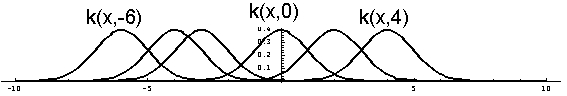
\includegraphics[width=0.8\columnwidth]{figures/kernel-fns-1}
\par\end{center}

\item Predictions of the form $f(x)=\sum_{i=1}^{6}\alpha_{i}k(x_{i},x)$:
\begin{center}
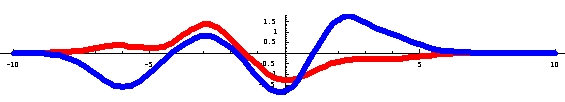
\includegraphics[width=0.8\columnwidth]{figures/kernel-fns-2}
\par\end{center}

\item When kernelizing with RBF kernel, prediction functions always look
this way (whether we get $w$ from SVM, ridge regression).
\end{itemize}
\end{frame}

\begin{frame}
    {Effect of the bandwidth}
    How does the fitted function change when we vary the bandwidth parameter?
    \pause
    \begin{figure}
        \begin{subfigure}[b]{0.3\textwidth}
            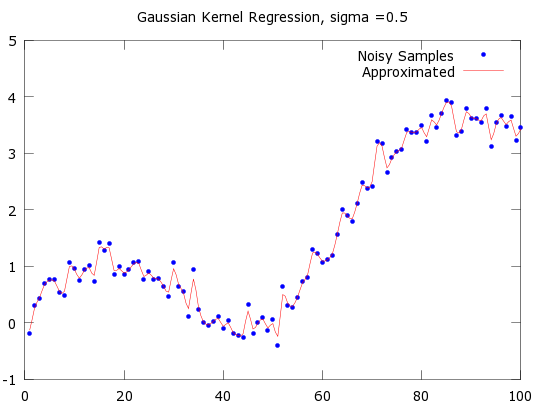
\includegraphics[width=\textwidth]{figures/2d_approx_sigma0_5}
            \caption{$\alpha=0.5$}
        \end{subfigure}
        \begin{subfigure}[b]{0.3\textwidth}
            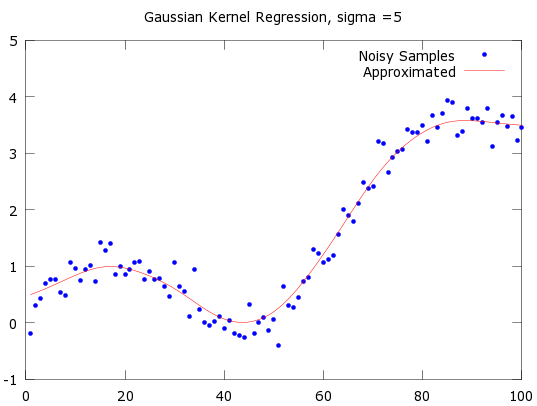
\includegraphics[width=\textwidth]{figures/2d_approx_sigma5}
            \caption{$\alpha=5$}
        \end{subfigure}
        \begin{subfigure}[b]{0.3\textwidth}
            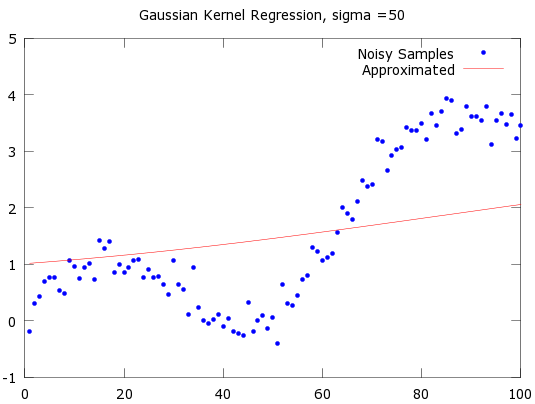
\includegraphics[width=\textwidth]{figures/2d_approx_sigma50}
            \caption{$\alpha=50$}
        \end{subfigure}
    \end{figure}

\let\thefootnote\relax\footnotetext{\url{https://mccormickml.com/2014/02/26/kernel-regression/}}
\end{frame}

\begin{frame}
    {Feature map of RBF kernel}
    What feature map corresponds to the RBF kernel?

    Consider the 1D case ($x\in\reals$) where $\sigma=1$:
    \begin{align}
        k(x,x') &= \exp\p{-\frac{(x-x')^2}{2}} \\
             &= \exp\p{-\frac{x^2}{2}}
             \exp\p{xx'}
             \exp\p{-\frac{{x'}^2}{2}}
    \end{align}
    \vspace{7em}
    \note[item]{Given
        \begin{align}
            k(x,x') &= \exp\p{-\frac{(x-x')^2}{2}} \\
             &= \exp\p{-\frac{x^2}{2}}
             \exp\p{xx'}
             \exp\p{-\frac{{x'}^2}{2}}
        \end{align}
    }
    \note[item]{
        We can also prove here that the Gaussian kernel is PD.
        The first and the third term is a 1D feature map, so their product is a PD kernel.
        The middle term is $\exp^{\pa{x,x'}}$, which is also a PD kernel.
        We can prove $\exp^{k(x,x')}$ is a kernel by writing $e$ as a power series, then each term in the sum is a product of valid kernels.
    }
    \note[item]{
        Now we only need to make the middle term separable in $x$ and $x'$, i.e. $\exp\p{xx'} = g(x)g(x')$.
    }
    \note[item]{
        Recall that $$e^x := \sum_{k=0}^\infty \frac{x^k}{k!}$$.
    }
    \note[item]{
        So we have $g(x)_k=\frac{x^k}{\sqrt{k!}}$ and $e^{xx'} = \sum_{k=0}^\infty g(x)_k g(x')_k$.
    }
    \note[item]{
        $$
        \phi(x)_k = \exp\p{-\frac{x^2}{2}} \frac{x^k}{\sqrt{k!}}
        $$
    }

\let\thefootnote\relax\footnotetext{Based on \url{https://www.cs.ubc.ca/~schmidtm/Courses/540-W19/L12.5.pdf}}
\end{frame}

\section{Kernel Methods}
\begin{frame}
    {Kernelization}
    \begin{itemize}
        \item A method can be kernelized if both training and inference only need inner produc in the feature space.
        \item Representer theorem says that all norm-regularized linear models can be kernelized.
            \note[item]{Note that the norm is induced by the Hilbert space.}
            \begin{itemize}
                \item Although we might be in a high dimensional space, $w$ lies in the subspace spanned by $\phi(x_i)$.
                \item Dimension of the subspace grows with the dataset size.
            \end{itemize}
        \item Many other algorithms can be kernelized.
    \end{itemize}
\end{frame}
% Other kernel methods
\begin{frame}
    {Kernelized perceptron}
    \begin{itemize}
        \setlength\itemsep{1ex}
        \item Initialize $w \leftarrow 0$
        \item While not converged
            \begin{itemize}
                \item For $(x_i, y_i)\in\sD$
                    \begin{itemize}
                        \item If $y_i w^Tx_i < 0$
                        \item Update $w \leftarrow w + y_ix_i$
                    \end{itemize}
            \end{itemize}
    \end{itemize}
    \note[item]{Show that $w$ is in the span of data by induction: each update leaves $w$ in the span of data.}
    \note[item]{Prediction: $$
    w\cdot x = \sum_{i=1}^n \alpha_i x_i\cdot x = k_x^T\alpha
    $$}
    \note[item]{
        Training: $\alpha_i \leftarrow \alpha_i + y_i$
    }
\end{frame}

\begin{frame}
    {Other kernel methods}
    \begin{itemize}
        \item Distance-based methods depending on $\|x-x'\|^2$
            \begin{itemize}
                \item $k$-means clustering
                \item $k$-nearest neighbors
            \end{itemize}
            \note[item]{
                $$
                \|x-x'\|^2 = \pa{x-x', x-x'} = \pa{x,x} - 2\pa{x,x'} + \pa{x',x'}
                $$
            }
        \item Eigenvalue methods: can show that eigenvector is in the span of data
            \begin{itemize}
                \item Principal component analysis
                \item Spectral clustering
            \end{itemize}
    \end{itemize}
\end{frame}
% Large-scale kernel methods
% - SVM vs ridge (sparsity)
\begin{frame}
    {Kernel SVM vs ridge}
    \begin{itemize}
        \item For both kernel SVM and ridge regression, we make predictions by
    $$
    \hat{f}(x) = k_x^T\alpha^* = \sum_{i=1}^n \alpha^*_i k(x_i, x)
    $$
\item For SVM, we have sparsity in $\alpha^*$ from complementary slackness.
\item For ridge, we need to access all training examples.
\item For large-scale dataset, we may not be able to store/compute the kernel matrix.
    \begin{itemize}
        \item Large-scale kernel machines (e.g. \hyperlink{https://people.eecs.berkeley.edu/~brecht/papers/07.rah.rec.nips.pdf}{Random Features for Large-Scale Kernel Machines})
    \end{itemize}
    \end{itemize}


\end{frame}

\end{document}
